% Created 2015-08-28 Fri 12:43
\documentclass[11pt]{kuntz-hw}
\usepackage[utf8]{inputenc}
\usepackage[T1]{fontenc}
\usepackage{fixltx2e}
\usepackage{graphicx}
\usepackage{longtable}
\usepackage{float}
\usepackage{wrapfig}
\usepackage{soul}
\usepackage{textcomp}
\usepackage{marvosym}
\usepackage[nointegrals]{wasysym} % symbols
\usepackage{latexsym}
\usepackage{hyperref}
\tolerance=1000
\usepackage{graphicx}
\usepackage{amsmath}
\usepackage{amssymb} % For set naming (i.e. R^n)
\usepackage{subfig}
\usepackage{url}

\class{CS 6370 / ME EN 6225 Motion Planning}
\institute{University of Utah}
\title{Project 2: Sampling Based Planning}
\begin{document}
\maketitle
\vspace{-30pt}
\section*{Instructions}
All solutions should be uploaded via the assignment on Canvas.

\textbf{Submission:} Please submit two \textbf{separate} files: a \textbf{pdf} report and a zip file.

\textbf{PDF Report:} Place all written answers  to questions as well as any images or other output data used to explain your responses in a single PDF document. This should be clearly named Proj\emph{<number>}-answers.pdf, where number is the Project number (i.e. 2 for this assignment). Please make sure to write your name and uid at the top of the document!

\textbf{Zip File:} Your zip file should be named in the format \emph{<uid>}.zip where \emph{<uid>} is your Utah uid. The first level of the zip should contain a single folder with your uid as the name \emph{<uid>}. Please put the README.txt, code and other necessary files (e.g. map or environment files) in the zip file. The README.txt should be in the root directory of your submitted zip file which explains how to run the code submitted.

\section*{Sampling Based Planning (100 total points)}
We will focus this project on implementing and analyzing a few of the sample based planning methods discussed in class.

\begin{figure}[h]
  \centering
  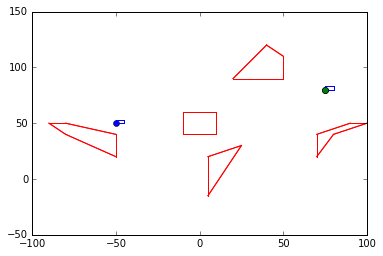
\includegraphics[width=0.6\textwidth]{env0}
  \caption{Environment 0 with start and goal configurations drawn.}
\end{figure}

\begin{figure}[h]
  \centering
  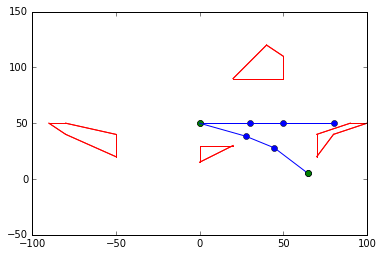
\includegraphics[width=0.6\textwidth]{env1}
  \caption{Environment 1 with start and goal configurations drawn.}
\end{figure}

To help you get started there is an included python file \texttt{collisions.py} which has some classes defined to help you focus on the algorithm implementation. There is an additional file named \texttt{Python\_Tips.pdf} on Canvas which gives some links and simple examples to help people who are new to python. The code also contains function headers for the search methods you need to implement. Feel free to change the function arguments necessary to make it easier for you to solve the problems. There are two environments provided in the files \texttt{env0.txt} and \texttt{env1.txt}, these define the robot parameters, the robot location, and a set of obstacles. They also provide a default start and goal position, but your implementation should be able to change these values when necessary.

Your planner should be general to work between both the environments. The first one uses a simple box robot that can only translate, while the second environment has an RRR robot with a fixed base. We will focus on planning in the 2D plane were we have polygonal objects, which makes collision checking easy to implement. We've provided a simple robot class for the box robot and RRR robot, which we will be using for the experiments. There is also a class that defines the environments and provides collision checking and simple visualization functions in \texttt{collisions.py}. We've also provided \texttt{rrt.py} which has a tree structure you can use in building your RRT, as well as some empty functions to fill out. Similarly we provide a \texttt{prm.py} containing the required data structures for implementing PRM


\section*{Rapidly-Exploring Random Trees (50 Points)}
\textbf{Note: If you are using Spyder, you will want to change Tools -> Preferences ->IPython console -> graphics backend to automatic to get the plots to work properly.} The inline option doesn't handle updating plots correctly.
\begin{description}

\item[Implement RRT] We'll start with implementing a traditional RRT and then build upon that with a few extensions. I should be able to run your code using a map file as described above and it should be clear how to change the transition function and actions used. You will need to be able to visualize the RRT tree and resulting plan/path for evaluation. For the three link robot, you can show a tree of the end-effector positions, to make visualization easier to understand. These functions are provided in the \texttt{PolygonalEnvironment} class.
It may be helpful to first plan and visualize these methods using a point in 2D space instead of with the full robot.

\item[1.1] (20 pts) Implement an RRT. Use the two environments provided to plan a path from init to goal. Sample toward the goal instead of a random sample with 5\% probability. Provide an image of both your tree and the resulting plan your algorithm finds for running on env0. Supply images of the resulting plan execution for env1.

For help debugging, our implementation produced a plan on env0 in about 1.8 seconds with a step size of 2.
For env1 we used a step size of 0.15 and needed at least 5000 samples to get a plan, but sometimes more samples. This would sometimes take over 2 minutes to run.

Run your RRT for both environments again with three, significantly different start and goal positions for each and again provide images of the tree and plan as before.

\item[1.2] (10 pts) Compare the trees and plans produced by sampling toward the goal with 0\%, 5\%, 10\%, and 50\% probability for env0.

\item[1.3] (10 pts) Extend your RRT implementation to create an RRT connect, replacing the standard \texttt{build\_rrt()} function with \texttt{build\_rrt\_connect()} which continues to extend towards a given sample instead of only making a single \(\epsilon\) length step until a collision occurs. Compare the resulting tree from running RRT-Connect to running the standard RRT for both env0 and env1. Use a 5\% goal sampling bias for both versions. Again provide the images of resulting tree and plan found by your algorithm.

\item[1.4] (10 pts) Now using your RRT connect implementation build a bi-directional RRT where you build two RRT-connects alternatively growing each one. Replace growing toward the goal with growing toward the other tree. Compare the resulting graph / trees and plan found to those found in the other versions above.
\end{description}

\section*{Probabilistic Roadmaps (30 Pts)}
\begin{description}
\item[Implement PRM] You now need to implement a PRM using the same robot and map models as above. Use a simple straight-line planner that checks collisions at a step size of \(\epsilon\) for a local planner (hint use epsilon equal to what worked well for your RRT).

\item[2.1] (30 pts) Implement the standard PRM using the same robots and environment as above. Build the PRM on the same maps, but now show results for planning with multiple start and goal locations, while building only a single roadmap. Show the roadmap built before attaching goals and initial positions, as well as the plans found for each of the different test situations. How does the resulting map change with different number of samples? How about changing the radius for Rdisk?

\item[2.2] \textbf{BONUS 15 pts} Now use your standard RRT implementation from problem 1 as the local planner in your PRM. Provide an image of your resulting roadmap. How does changing the number of samples change the performance of the PRM with an RRT local planner? How does the radius affect performance?
\end{description}


\section*{CoppeliaSim  7Dof arm (15 Pts)}
\begin{description}
\item[Setup]You first need to download CoppeliaSim 4.1.0 and get it running on your system. \textbf{If you encounter problems, please post them to the Discussion board}, because it is likely that others will have the same problem. Follow these steps: 

Download CoppeliaSim Edu 4.0 / 4.1 (more recent versions are not compatible with the code base) for your operating system:  \href{https://www.coppeliarobotics.com/files/CoppeliaSim_Edu_V4_0_0_Setup.exe}{Windows}, \href{https://www.coppeliarobotics.com/files/CoppeliaSim_Edu_V4_0_0_Mac.zip}{Mac}, or Ubuntu \href{https://www.coppeliarobotics.com/files/CoppeliaSim_Edu_V4_1_0_Ubuntu18_04.tar.xz}{18.04} \href{https://www.coppeliarobotics.com/files/CoppeliaSim_Edu_V4_1_0_Ubuntu20_04.tar.xz}{20.04/22.04} (Links inline). For Mac this is a zip file, for Linux it is a tarball, and for Windows it is a setup executable.
	
Install CoppeliaSim on your system. For Mac and Linux you simply have to expand the compressed file you downloaded to a directory of your choosing and you're ready to go. For Windows you have to run the setup executable and it will install where you tell it on your system.
	
Navigate to the CoppeliaSim root folder and start the application: \texttt{coppeliaSim.app} in Mac, \texttt{coppeliaSim.sh} in Linux, \texttt{coppeliaSim.exe} in Windows. You should see an empty environment come up:

\textbf{Note the simulator used to be called VREP so our internal files will refer to it as VREP}

Go to your running instance of CoppeliaSim and open the environment we provide by going to \texttt{File > Open Scene...} and navigating to the file \\ \texttt{project2/vrepfiles/vrepfiles/lbr4\_environment.ttt}. You should see an LBR4 robot arm with a Barrett Hand come up.


\item[Common Issues] Past students have resolved CoppeliaSim problems, described below

1. Students have had issues importing vrep.py because python was 32bit version. If you have this issue reinstall with 64bit version of python.

2. If the simulator throws a 'libpython3.5.so.1 not found', setup a conda environment with python3.5 and it to the library path and relaunch the simulator.

\item[Simulated Robot] You now need to run your RRT implementation on the CoppeliaSim simulated robot. Run the \texttt{lbr4\_testscript.py} to verify your computer is setup correctly, expect experiments to take 1-5 minutes.


\item[3.1] (5 pts) Run normal RRT with CoppeliaSim robot. Show screenshot of CoppeliaSim.
\item[3.2] (5 pts) Run RRT connect with CoppeliaSim robot. Show screenshot of CoppeliaSim.
\item[3.3] (5 pts) Run bidirectional RRT connect with CoppeliaSim robot. Show screenshot of CoppeliaSim.
\end{description}

\section*{Self Analysis (5 pts)}
\begin{description}
\item[4.1] (1 pt) What was the hardest part of the assignment for you?
\item[4.2] (1 pt) What was the easiest part of the assignment for you?
\item[4.3] (1 pt) What problem(s) helped further your understanding of the course material?
\item[4.4] (1 pt) Did you feel any problems were tedious and not helpful to your understanding of the material?
\item[4.5] (1 pt) What other feedback do you have about this homework?
\end{description}

\end{document}
